
\section{Desarrollo}

Después de haber realizado el análisis inicial de el alcance del proyecto y las necesidades de los usuarios, se comenzó con el desarrollo del proyecto. Este desarrollo se hizo en tres partes. Primero, el desarrollo de un módulo de monitoreo de las estaciones meteorológicas por medio de drivers,  después un API como intermediaria entre la información almacenada en la base de datos y una interfaz gráfica para el monitoreo eficaz.

\subsection{De la base de datos}

Debido a que se seleccionó un sistema basado en un ORM para el manejo de la base de datos, esta tiene que modelarse en el sistema en forma de código para ser reconocida, de la misma forma, la creación de la estructura de la base de datos en el motor se hará por medio de migraciones creadas con el sistema de creación de base de datos, para facilitar su mantenimiento e interoperabilidad en diferentes sistemas y facilitar las integraciones con otros sistemas existentes de información.

Los archivos resultantes de estas migraciones fueron tal como se muestran en el Listado \ref{lst:database-migrations-files}, las cuales se pueden encontrar en la ruta \texttt{/app/database/migrations} del proyecto, tal como es especificado en las guías de desarrollo de MasoniteORM.

\begin{listing}
\begin{minted}{bash}
2021_08_03_052340_stations.py
2021_10_14_162126_station_additional.py
2021_11_13_020934_event_solutions.py
2022_04_03_003436_add_timestamps.py
2021_08_16_000028_station_events.py
2021_10_29_035514_stations.py
2022_03_25_013638_normalize_events_comments.py
2022_04_20_222630_events_fix.py
\end{minted}
\caption{Archivos de migración en el proyecto.}
\label{lst:database-migrations-files}
\end{listing}

Si bien los modelos creados para la ejecución de este proyecto siguen los estándares de modelado de base de datos especificados en MasoniteORM, tal que al modelar la base de datos es posible obtener el mismo código que el implementado, una modificación importante al modelado de los datos es el uso de un mutador para traducir las direcciones IP a enteros y viceversa. Este mutador es accesado con un nombre alternativo al nombre del campo en el modelo, debido a que por limitaciones del ORM no es posible utilizar mutadores y accesores con el mismo nombre del campo objetivo. En el Listado \ref{lst:model-station-mutator} es posible observar el mutador mencionado y su definición, cabe resaltar que la presencia de los caracteres \texttt{[...]} indican que existe más código con otras funcionalidades que se omitió por fines de brevedad.

\begin{listing}
\begin{minted}{python}
import ipaddress
[...]
class Station(Model, UUIDPrimaryKeyMixin, SoftDeletesMixin):
[...]
def get_ip_address_attribute(self):
   return str(ipaddress.ip_address(self.ip))

def set_ip_attribute(self, attribute):
   try:
      ip = ipaddress.ip_address(attribute)
   except ValueError:
      raise ValueError("Invalid IP Address %s" % attribute)

   return int(ipaddress.ip_address(attribute))
\end{minted}
\caption{Definición de accesor y mutador para modelo de estaciones.}
\label{lst:model-station-mutator}
\end{listing}

\subsubsection{Selección del motor de base de datos}

Para el caso de uso del centro de monitoreo de estaciones meteorológicas de la UACJ, en el que la red actual cuenta con 13 estaciones, no es necesario considerar como cuello de botella el motor de base de datos que se utilizará para el sistema. Esto debido a que, con un tiempo mínimo para la consulta del estado de las estaciones de hasta 5 minutos entre consultas, el sistema podría funcionar incluso con un tiempo promedio de 23 segundos desde la consulta hasta el almacenamiento de la información. Esto, sin tomar en cuenta que es posible paralelizar el proceso de consulta y generación de eventos de las estaciones meteorológicas, por lo que no se considera como algo relevante la selección de un motor de base de datos que cuente con alto rendimiento de lectura y/o escritura de la información.

Debido a que la infraestructura del sistema de las estaciones meteorológicas ya utiliza un motor relacional de base de datos adecuado para el proyecto, MySQL, se pretende utilizarlo para este proyecto, reduciendo la carga de mantenimiento para el equipo de la universidad, además de un sistema familiar que permitirá a los involucrados realizar consultas a la información sin necesidad de aprender nuevas tecnologías.

Para esto, se utilizó la flexibilidad que ofrecen los sistemas modelado de objetos y roles (ORM, por sus siglas en inglés) \cite{Halpin2006}, en la que se permite el crear sistemas agnósticos de un motor de base de datos en específico, y la creación de modelos, esquemas y relaciones de base de datos se dejan al \textit{framework} de modelado de datos. Esto además ofrece soporte para migraciones para realizar actualizaciones de base de datos controladas en caso de requerir extender un sistema existente.

El motor de base de datos seleccionado para el desarrollo local del proyecto fué \textit{SQLite}, debido a la flexibilidad que ofrece al ser una base de datos que sólo depende de un archivo para funcionar y que no requiere de la instalación de paquetes de software extra en la estación que se utiliza para desarrollar y probar el proyecto.


\subsection{Del módulo de monitoreo de las estaciones}

Para realizar el monitoreo a las estaciones meteorológicas, se decidió dividir el módulo en dos componentes principales, un submódulo de generación de reportes y un sistema de controladores que contuvieran el código de conexión y restauración de servicios de las estaciones.

Tomando como referencia el proyecto de \textit{Monitoring Plugins} \cite{monitoring_plugins}, el cual es compatible con diversos proyectos especializados en monitoreo de sistemas de alta resilencia, tales como \textit{Nagios} y \textit{Icinga}, se decidió crear un proyecto basado en drivers que pudieran ser extendibles. Cada uno de estos drivers, puede cargar una cantidad \textit{n} de módulos o servicios, que contienen la información necesaria para obtener el estado de la estación meteorológica y generar un reporte que contenga información comprehensiva del estado de las estaciones.

Con el objetivo de crear un sistema que fuera posible integrar en diferentes ambientes y no requiriera de previa instalación de componentes extra en el dispositivo objetivo, se decidió que la técnica con cual se revisaría el estado de las estaciones es por medio de un comando que se ejecutaría en una estación remota, o de forma local dado el caso, y se comparara la respuesta obtenida con el resultado de la operación. En caso de que la respuesta de esta operación sea diferente a la respuesta esperada, se buscaría en un arreglo de casos conocidos, que pueden ser solucionados con la ejecución de un comando.
Debido a esto se utilizó una estructura de

Debido a que es necesaria más información que sólo el comando que se requiere ejecutar en una estación, se decidió crear una estructura basada en servicios para el monitoreo de las estaciones. Además, de esta forma, un controlador de una estación podría reutilizar fácilmente servicios que fueran utilizados en controladores para el monitoreo de otras estaciones, tal como es el estado de la base de datos y otros similares.

La estructura del servicio resultante es un objeto en el lenguaje Python con la forma que se puede apreciar en el Listado \ref{lst:service-example}, donde el arreglo de casos conocidos tiene el nombre de \textit{actions}, y es anidable, lo que permite listar una serie de comandos que pueden ayudar a la solución de problemas con una produndidad \textit{n}.

\begin{listing}
\begin{minted}[%
   breaklines
]{python3}
service = {
   "command": "", # Comando a ejecutar
   "stdout": "", # Salida esperada
   "stderr": "", # Error esperado
   "actions": {
      "read_write_enabled": {
         "response_stdout": "", # Si la respuesta del comando previo es esta
         "response_stderr": "", # Si el error del comando previo es este

         "description": "", # Descripción para el usuario del error
         "solution": "", # Solución propuesta, si existe, para el usuario

         "command": "", # Comando a ejecutar
         "stdout": "", # Salida esperada
         "stderr": "", # Error esperado
         "actions": {
            # ...
         }
      }
   }
}
\end{minted}
\caption{Ejemplo de estructura de un servicio.}
\label{lst:service-example}
\end{listing}

Para el desarrollo de la estructura del controlador de monitoreo de las estaciones meteorológicas, se optó por crear un sistema orientado a la extensión de un componente base que fungiera como sistema principal de ejecución, verificación de credenciales y ejecución de comandos en el sistema objetivo. La estructura de los controladores resultante es que cualquier módulo puede contener una serie de controladores relacionados, y cada uno de estos controladores extiende un driver base para hacer uso de diversas funciones, como el obtener información o registrar la estación. La estructura implementada resultante puede ser observada en la Figura \ref{fig:diagrama_clase_drivers}.

\begin{figure}[!ht]
	\centering
	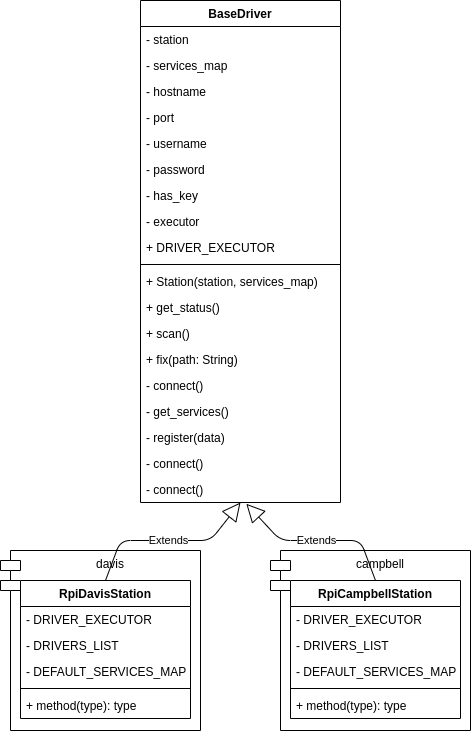
\includegraphics[width=0.5\linewidth]{images/diagrams/classes/drivers.drawio.png}
	\caption{Diagrama de clase de controladores}
	\label{fig:diagrama_clase_drivers}
\end{figure}

Debido a que este diseño de controlador requiere de ser instanciado cada vez que se busca obtener la información más reciente, esto permite el crear servicios más complejos que la estructura mencionada anteriormente, un ejemplo es la implementación del servicio de control de la fecha y la hora de la estación, que impide que esta sea desvíe por más de 15 minutos de la hora del sistema de monitoreo, para asegurar la calidad de los datos recabados. En este caso, se hace uso de la librería \texttt{time} de Python para obtener la hora actual en formato Unix, para después compararla por medio de bash con la hora del sistema objetivo.

La implementación de el servicio mencionado anteriormente puede ser observada en el listado \ref{lst:time_service}, sin embargo, cabe notar que es posible escribir otro tipo de estructuras de servicios, tales como clases, funciones como en este caso, e incluso ser generado con una base de datos.

\begin{listing}
\begin{minted}[%
   breaklines
]{python3}
import time

def service():
  # Get's and compares the datetime against the current time in bash
  command = 'CURRENT=$(date +%s); MINUTES=$(( ({0} - $CURRENT) / 60 ));'.format(int(time.time()))

  # Checks if the obtained minutes is greater than 15 minutes, prints true if it is.
  command += 'if (( $MINUTES > 15 || $MINUTES < -15 )); then echo "true $MINUTES"; else echo "false $MINUTES"; fi'

  service = {
   "command": command,
   [...]
  }

  return service
\end{minted}
\caption{Ejemplo del servicio para revisión de tiempo.}
\label{lst:time_service}
\end{listing}

Para poder estandarizar la ejecución de los comandos en diversos tipos de sistemas, se creó un módulo que por medio de interfaces estandariza la ejecución, si es proveído con la información necesaria para realizar la tarea. Para esto, se creó una clase de ejecutor base de la cual surgen un ejecutor local y uno remoto, el último de estos requiriendo una serie de elementos, como credenciales y un \textit{host} destino para su funcionamiento. El diagrama de clase que representa el código resultante puede ser visto en la Figura \ref*{fig:diagrama_clase_ejecutores}.

\begin{figure}[!ht]
	\centering
	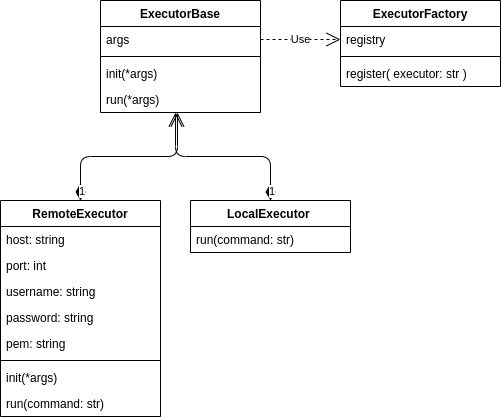
\includegraphics[width=0.7\linewidth]{images/diagrams/classes/executors.drawio.png}
	\caption{Diagrama de clase de ejecutores.}
	\label{fig:diagrama_clase_ejecutores}
\end{figure}

Esta implementación puede facilitar la creación de más ejecutores para casos de uso específico, como un ejecutor para un sistema que dependa de la comunicación por puertos seriales, gracias a la capacidad de registrar nuevos ejecutores en la fábrica sin necesidad de reescribir el código existente.

El módulo de monitoreo tiene como objetivo principal el observar la información obtenida por los diversos controladores y generar reportes conforme sea adecuado. Durante este proceso, se toman los datos de una estación y se utilizan para crear una conexión a la estación para obtener la información con un controlador. Este controlador utiliza un ejecutor para enviar los comandos en la definición de los múltiples servicios a la estación, y regresa un arreglo estandarizado que contiene la información de los problemas que se encontraron al realizar el proceso, tal como se muestra en la Figura \ref{fig:diagrama_secuencia_de_monitoreo}.

\begin{figure}[!ht]
	\centering
	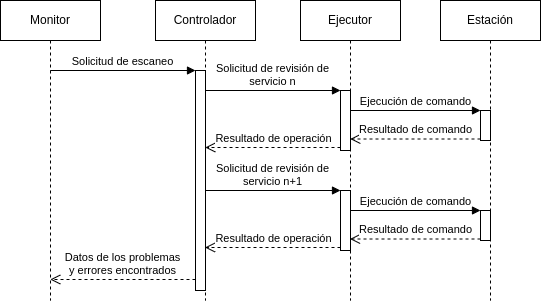
\includegraphics[width=0.9\linewidth]{images/diagrams/classes/monitoring_diagram.drawio.png}
	\caption{Diagrama de secuencia para el monitoreo de las estaciones.}
	\label{fig:diagrama_secuencia_de_monitoreo}
\end{figure}

El módulo de monitoreo después toma la información obtenida para ser guardada en base de datos y generar los eventos conforme a la configuración del proyecto. Cabe notar que sólo se recaba la información de los servicios que han sido detectados con algún problema, esto se hace para cumplir con el objetivo de maximizar el espacio de la base de datos discriminando la información que no se considera relevante.

Cuando uno de estos eventos es generado, se al sistema de notificaciones que se integró. Este sistema de notificaciones consiste de un archivo de configuración para obtener las credenciales necesarias para realizar operaciones, así como una clase interface que instancia el SDK del serivicio seleccionado ,en este caso OneSignal. La elección de OneSignal se debió a su previo uso en la Universidad Autónoma de Ciudad Juárez, así como por la existencia de una librería estándar en el lenguaje para interactuar con el servicio.

Estos procesos además de ser documentados en el presente documento, fueron documentados en el código con el estándar de \textit{docstrings} de Python, debido a esto fué posible generar una documentación automática del proyecto para una fácil navegación. Esta documentación fué generada con la libería \textit{pdoc} y la documentación que puede ser observada en la Figura \ref{fig:docs_station_reporter_lib}, fué generada ejecutando el comando \texttt{pdoc generate --html} en la estación de desarrollo.

\begin{figure}[!ht]
	\centering
	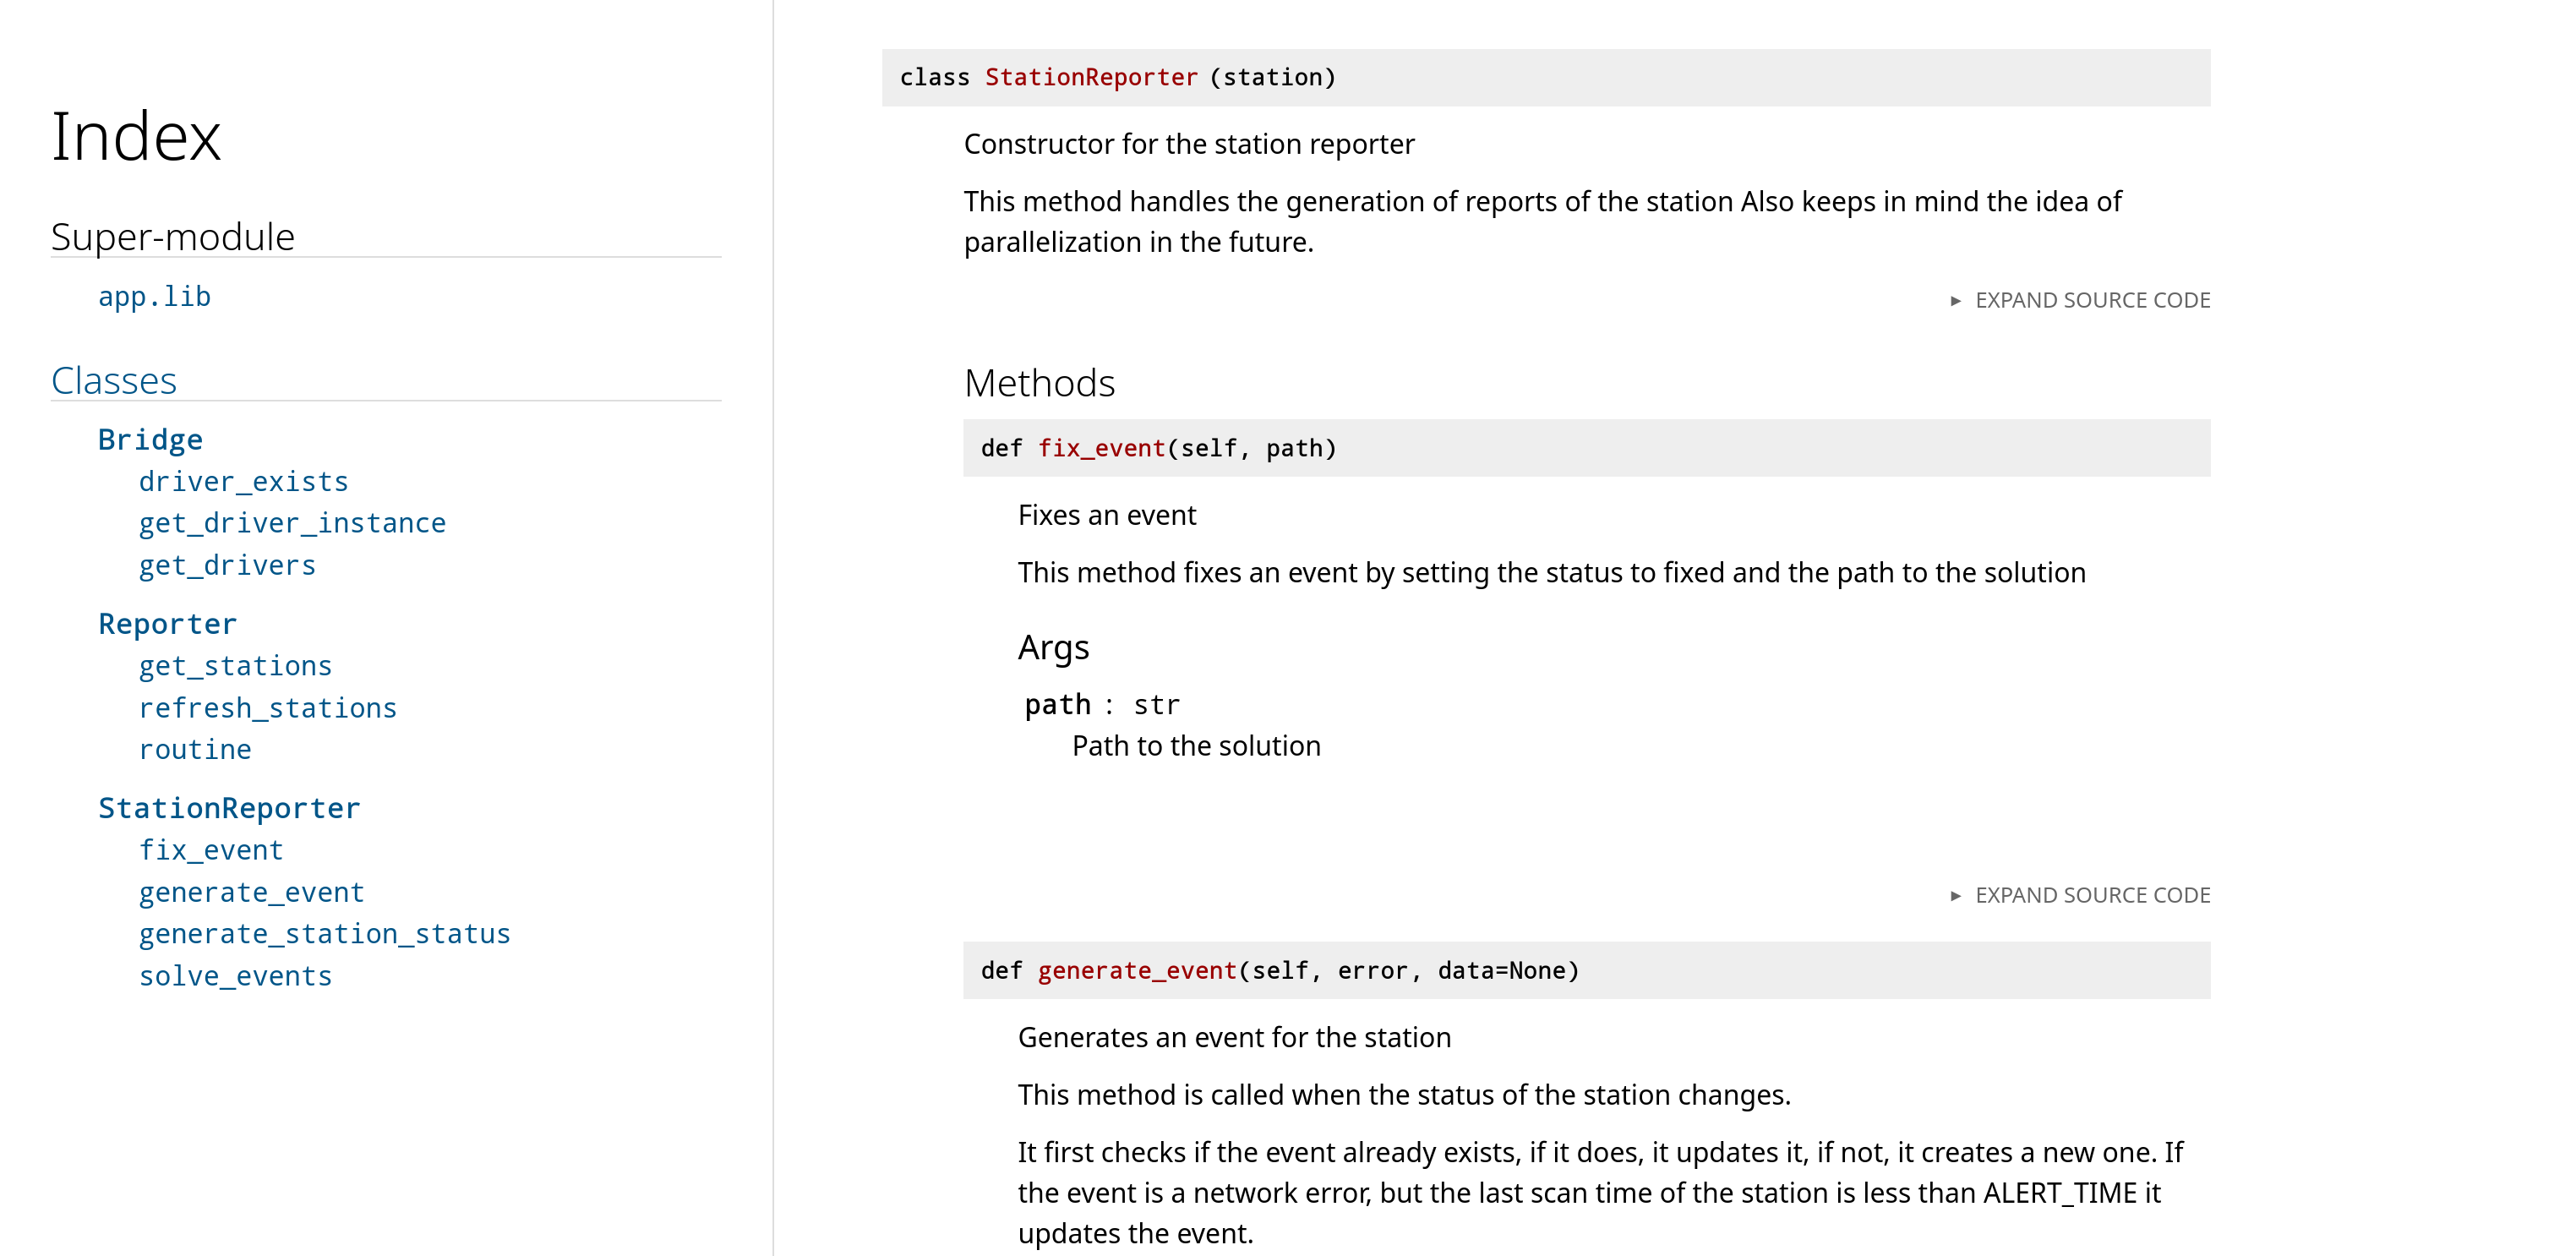
\includegraphics[width=1\linewidth]{images/screenshots/lib_docs_station.png}
	\caption{Captura de documentación de librería.}
	\label{fig:docs_station_reporter_lib}
\end{figure}

\subsubsection{Desarrollo de los servicios de monitoreo}

Un servicio fundamental para la longevidad de las estaciones meteorológicas, es el de \href{https://github.com/glennmckechnie/rorpi-raspberrypi}{RoPI}, este programa convierte la tarjeta SD de la estación meteorológica en un disco de sólo lectura, lo que reduce el estrés que esta sufre al estar funcionando y reduzca el riesgo de corrupción. Para el monitoreo de este servicio, se analizó el código de el servicio y se copió la misma instrucción que utiliza la herramienta para verificar el estado del sistema. En caso de que este servicio no esté funcionando, sólo se requiere reactivar el modo sólo lecutura. El servicio de monitoreo resultante es el que se puede observar en el Listado \ref{lst:ropi_service}

\begin{listing}
\begin{minted}[%
   breaklines
]{python3}
service = {
    "command": "echo $(awk '/root/{print $4}' /proc/mounts | awk -F , '{print $1}')",
    "stdout": "ro",
    "stderr": None,
    "actions": {
        "read_write_enabled": {
            "description": "La estación está en modo escritura",
            "solution": "Reactivar el modo sólo lectura",
            "response_stdout": "rw",
            "response_stderr": None,

            # Solution and the expected solution result
            "command": "sudo remountro",
            "stdout": None,
            "stderr": None,
        }
    }
}
\end{minted}
\caption{Ejemplo del servicio para revisión de RoPI.}
\label{lst:ropi_service}
\end{listing}

En el caso del servicio WeeWX, el encargado de recolectar la información de las estaciones con la ayuda de diversos métodos específicos, sólo es necesario verificar que el proceso que recolecta la información esté funcionando. Este proceso está configurado como un servicio de Linux, por lo cual es posible obtener su estado por medio de la herramienta de sistema \texttt{systemd}.

Entre las fallas comunes de este servicio, podemos encontrar una sobrecarga de la estación ocurrida cuando el servicio hace demasiados intentos de recolección al equipo destino sin enviar los terminadores adecuados. Para solucionar este problema, es necesario conectarse con la herramienta destinada a la conexión con los dispositivos y ejecutar una limpieza de memoria, con el comando \texttt{wee\_device --clear-memory}. Por último, cuando no sea posible ejecutar este comando por una conexión previa no finalizada al sistema, se desconecta forzozamente la conexión con las herramientas que Linux proporciona. Este proceso mencionado, se definió en el sistema de monitoreo de la forma que se muestra en el Listado \ref{lst:weewx_service}

\begin{listing}
\begin{minted}[%
   breaklines
]{python3}
# Check the WeeWX service
service = {
    "command": "systemctl status weewx",
    "stdout": "Active: active (running)",
    "stderr": None,  # None implica que esperamos que se encuentre vacío

    "actions": {
        "unable_to_wake": {
            "description": "Problema de conexión a la consola Davis por puerto serial",
            "solution": "Reinicia la memoria de la consola Davis por medio de la opción --clear-memory",
            "response_stdout": "vantage: Unable to wake up console",
            "response_stderr": None,
            "command": "sudo wee_device --clear-memory && sudo wee_device --info",
            "actions": {
                # There is no connection to clear the memory of the station
                "bad_serial": {
                        "description": "No tenemos conexión para limpiar la memoria de la estación",
                        "solution": "Reiniciar conexión serial",
                        "response_stdout": "OSError: [Errno 11] Resource temporarily unavailable",
                        "response_stderr": None,
                        "command": "sudo systemctl stop serial-getty@ttyS0.service"
                }
            }
        }
    }
}
\end{minted}
\caption{Ejemplo del servicio WeeWX.}
\label{lst:weewx_service}
\end{listing}


\subsection{Del API para el acceso a la información}

El API para el acceso a la información fue desarrollado con la ayuda de FastAPI y MasoniteORM. Estos fueron utilizados para proveer acceso a los estados de las estaciones, datos históricos, registros de datos, así como para la llamada a los controladores de las estaciones para operaciones especiales.

Debido a la arquitectura de FastAPI, el sistema se dividió en \texttt{routers}, \texttt{requests} y modelos. Todos estos son instanciados y llamados desde un archivo \texttt{main.py} que se encuentra en la ruta \texttt{/app/app/main.py}, conforme a las especificaciones de desarrollo estándar del framework. Además, en este archivo se especifican descripciones estándar generales que serán incluídas al autogenerar la documentación, tal como la de la Figura \ref{fig:openapi_redoc}, así como definiciones generales de acceso, permisos de CORS y definiciones globales de las rutas.

\begin{figure}[!ht]
	\centering
	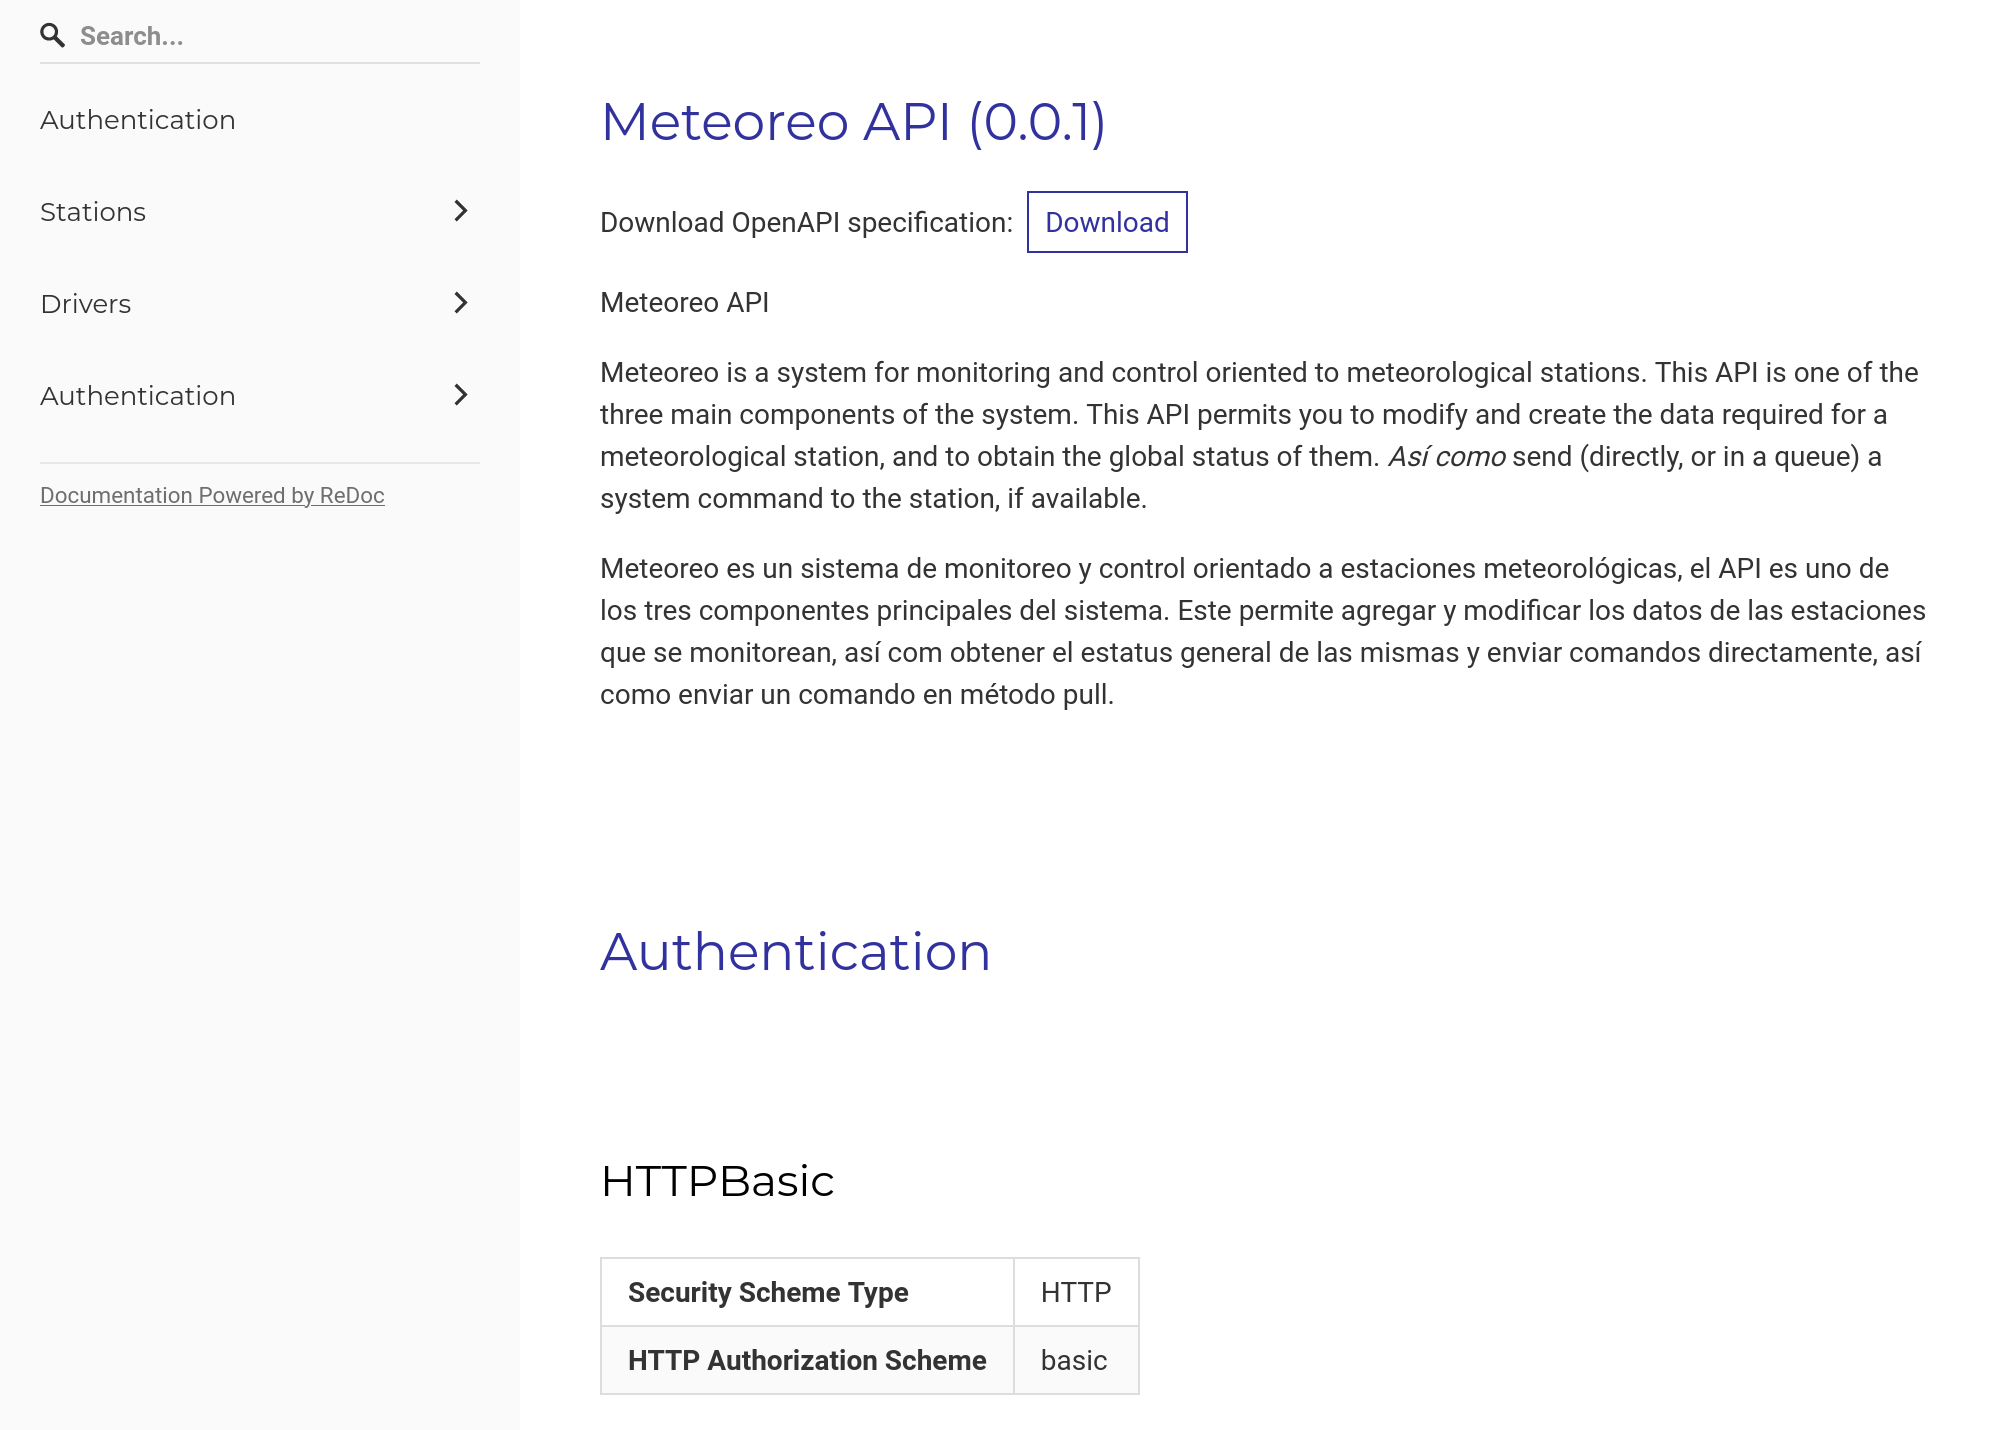
\includegraphics[width=1\linewidth]{images/screenshots/ReDoc_api_docs.png}
	\caption{Visualización de documentación en OpenAPI.}
	\label{fig:openapi_redoc}
\end{figure}

Para el manejo de la información, se crearon rutas para los módulos de autenticación, incidentes, controladores y estaciones. Estas rutas soportan operaciones CRUD básicas y existen rutas específicas para la interacción con algunos servicios, tal como es el caso del registro de estaciones que permite instanciar una instancia del controlador para registrar una nueva estación en el sistema.

Para el manejo de la información, se utilizó MasoniteORM de forma estándar como lo indica su documentación, aunque cabe notar que debido a limitaciones del framework y a que es utilizado con FastAPI, a pesar de que las definiciones de los modelos contienen las relaciones de la información necesarias estos tienen un problema al intentar ser serializados automáticamente por el framework al momento de ser llamados en una ruta, por lo que se tiene que hacer el llamado a la función \texttt{serialize()} de cada uno de los miembros en relación para cada una de las estaciones, esto resulta en código como el que puede ser observado en el Listado \ref{lst:events_serialization}.

\begin{listing}
\begin{minted}[%
   breaklines
]{python3}
from uuid import UUID
from ..models.Station import Station
[...]
@router.get("/{uuid}")
def get_station(uuid: str):
  """
  Get a specific station from it's uuid=
  """
  result = Station.find(uuid)
  result.incidents = result.events.serialize()

  return result.serialize()
\end{minted}
\caption{Serialización de datos con FastAPI y MasoniteORM.}
\label{lst:events_serialization}
\end{listing}

\subsection{De la interfaz gráfica del proyecto}

El desarrollo de la interfaz gráfica del proyecto pasó por una serie de iteraciones para poder llegar a un estado de calidad que se considerara adecuado para el proyecto. Estas iteraciones fueron realizadas de forma eficaz gracias a la arquitectura basada en componentes que ofrece Tailwind y VueJS, permitiendo reescribir sólamente partes del sistema cada vez que fuera requerido algo.

La estructura del proyecto se dividió en un router para la definición de las rutas que serían accesibles en el sistema, una carpeta de vistas que son incluídas desde el router para la generación de las estructuras principales de las páginas web a las que son necesarias acceder, y por útlimo una carpeta de componentes que permitiera el crear archivos individuales para la funcionalidad de los componentes que integran la aplicación.

La vista principal del sistema es una vista general de todas las estaciones tal como estaba definida en el capítulo de diseño (véase Figura \ref{fig:dashboard}), la cual ofrece un estado comprensivo de cada estación y que al seleccionar una estación, abre una segunda vista con información más específica de la estación, como puede ser observado en la Figura \ref{fig:station-failed}. Esta vista posee una cualidad reactiva, lo cual permite que los datos sean actualizados en la página sin necesidad de ejecutar una operación de recarga en el navegador en el que se está viendo.

\begin{figure}[!ht]
	\centering
	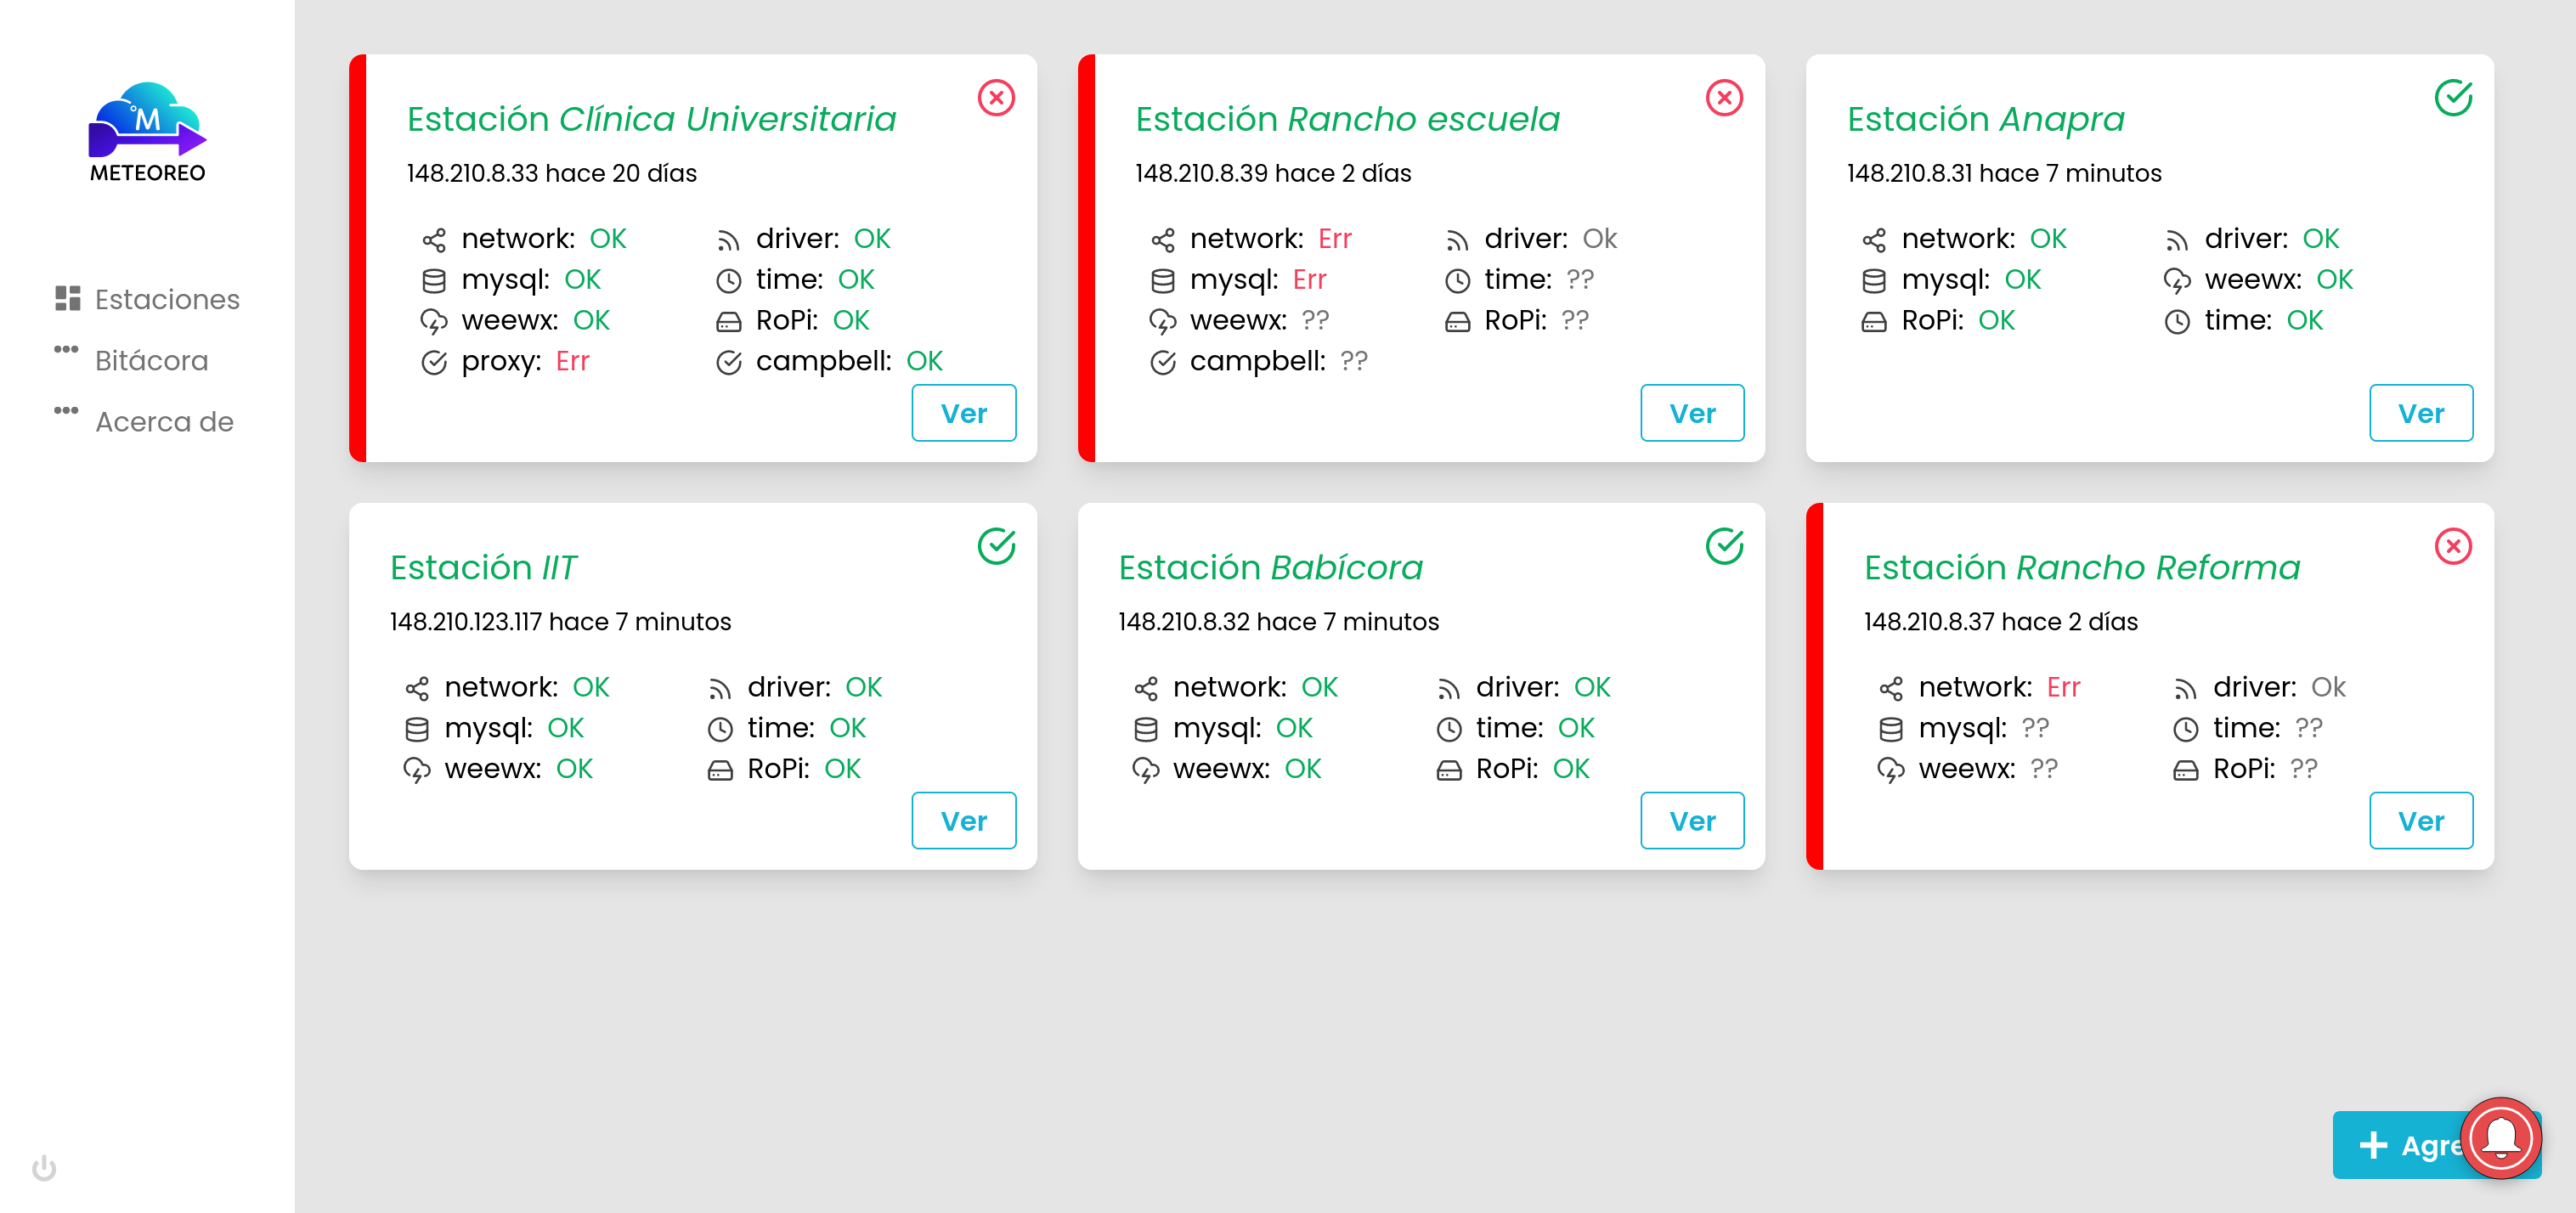
\includegraphics[width=1\linewidth]{images/screenshots/0.0.0-dashboard.png}
	\caption{Vista general de las estaciones.}
	\label{fig:dashboard}
\end{figure}

\begin{figure}[!ht]
	\centering
	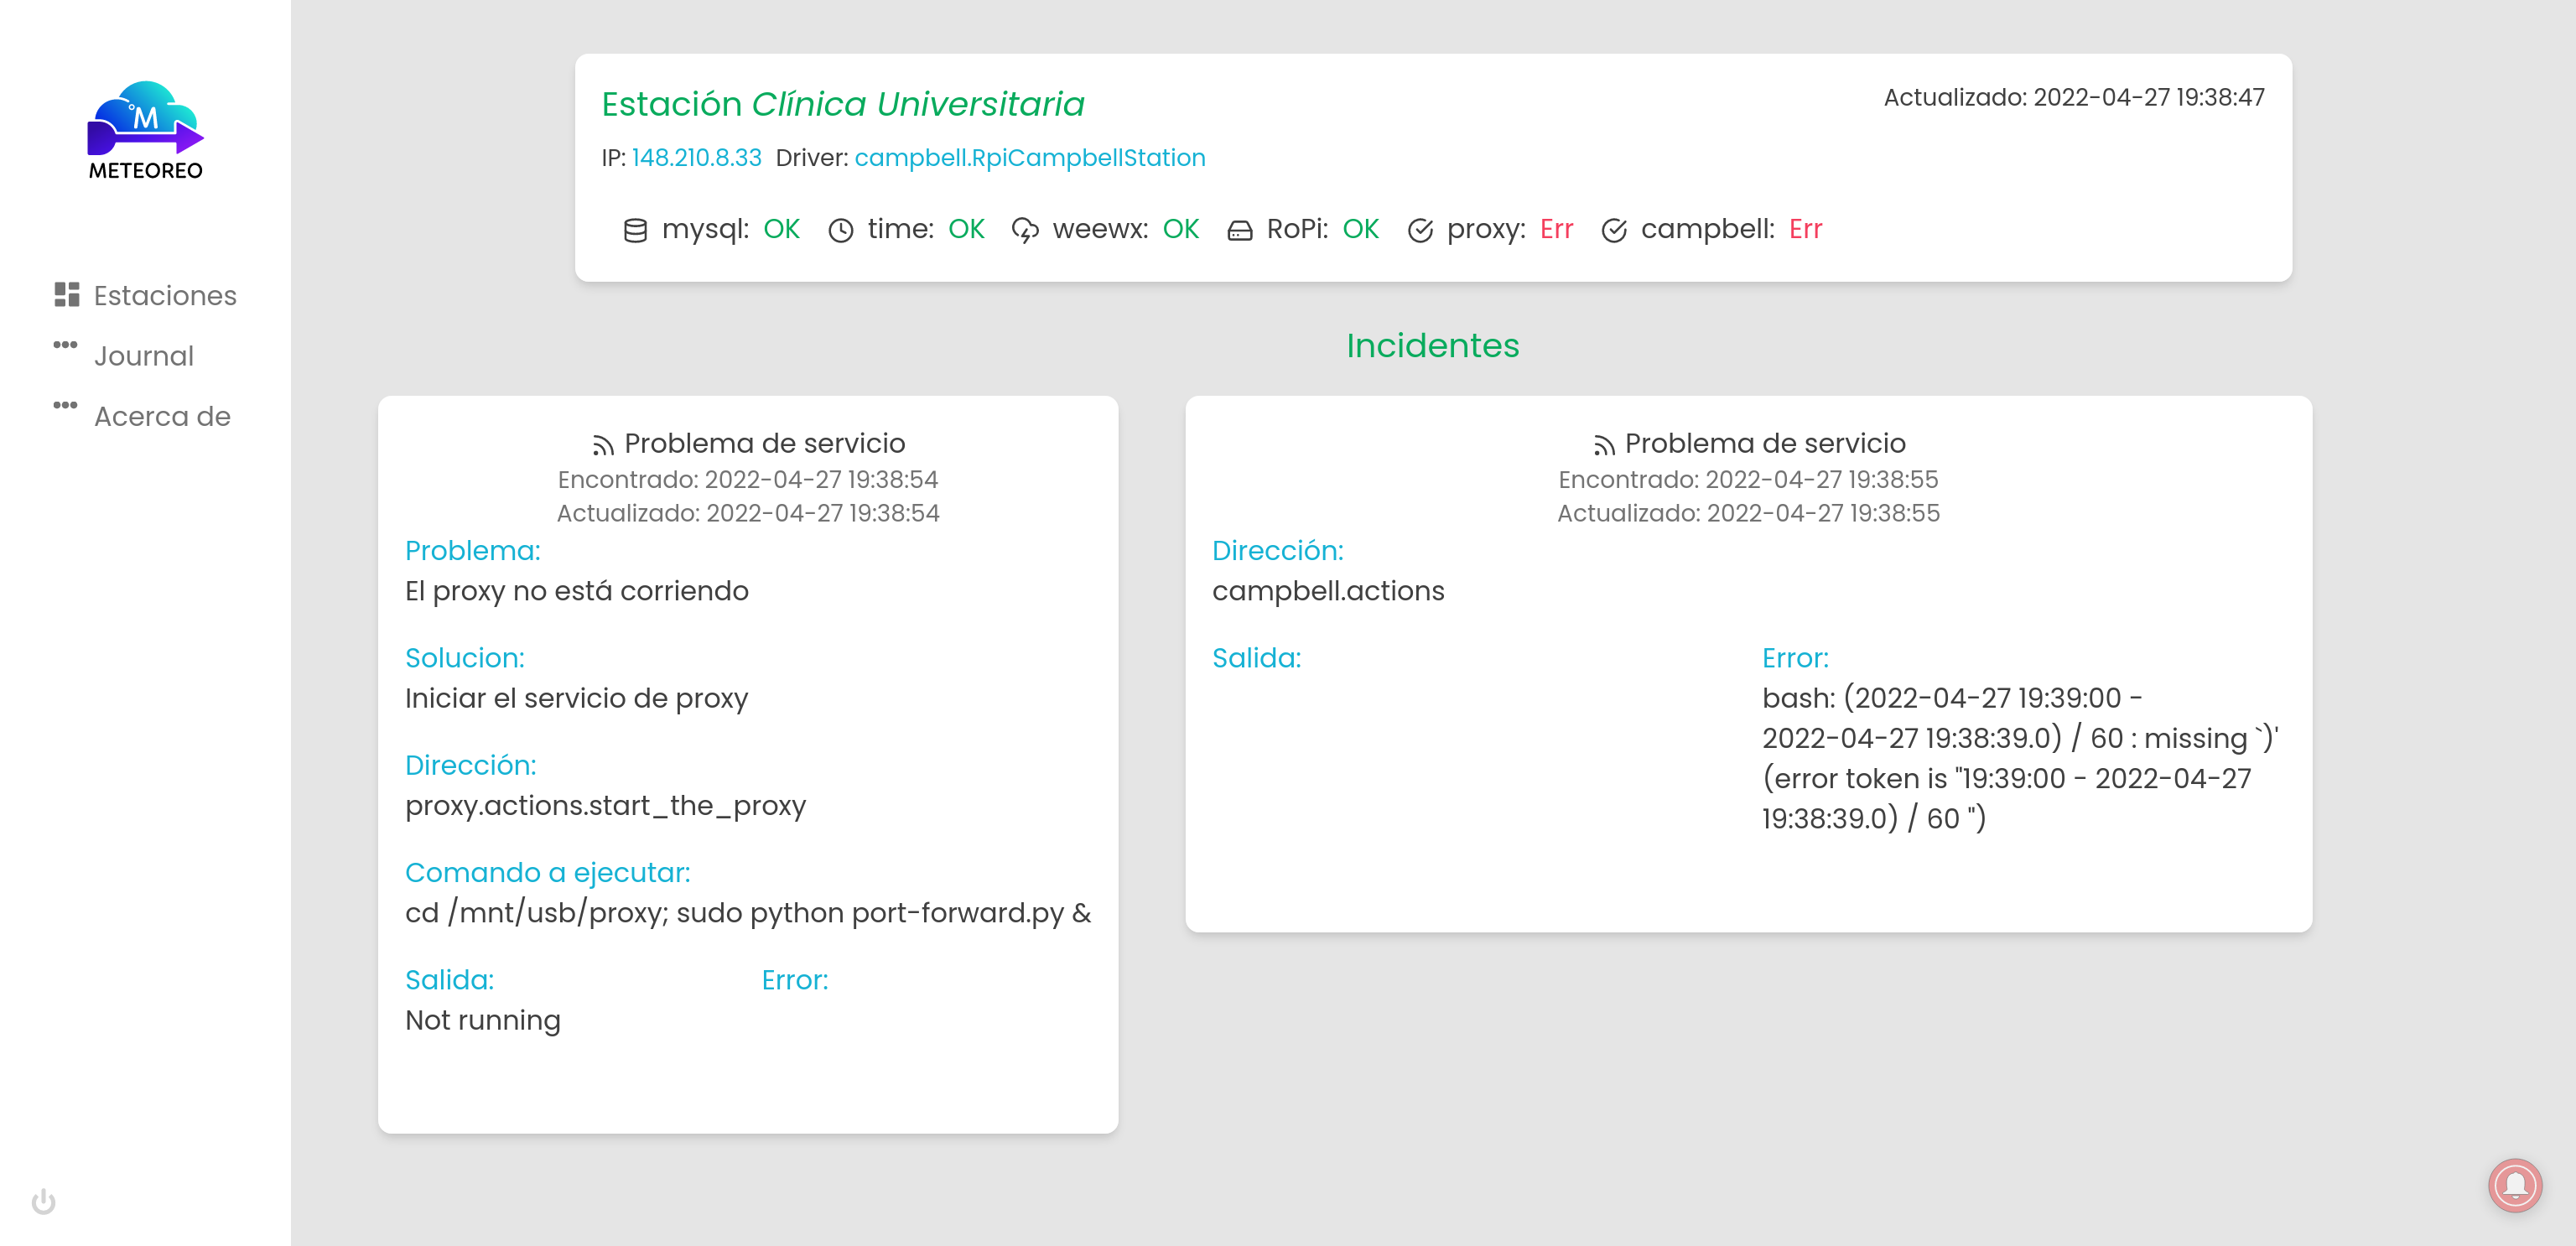
\includegraphics[width=1\linewidth]{images/screenshots/0.1.0-station_failed.png}
	\caption{Vista de una estación con fallas.}
	\label{fig:station-failed}
\end{figure}

Gracias a la cualidad adaptativa de Tailwind, que utiliza un sistema de puntos de ruptura orientado a la máxima eficacia en el desarrollo para móviles, el sistema resultante fue posible hacerlo compatible con estos sistemas con una cantidad mínima de esfuerzo, la interfaz resultante, que puede verse en la Figura \ref{fig:dashboard-responsive}, tiene una visualización adecuada en sitios que no son de escritorio.

\begin{figure}[!ht]
	\centering
	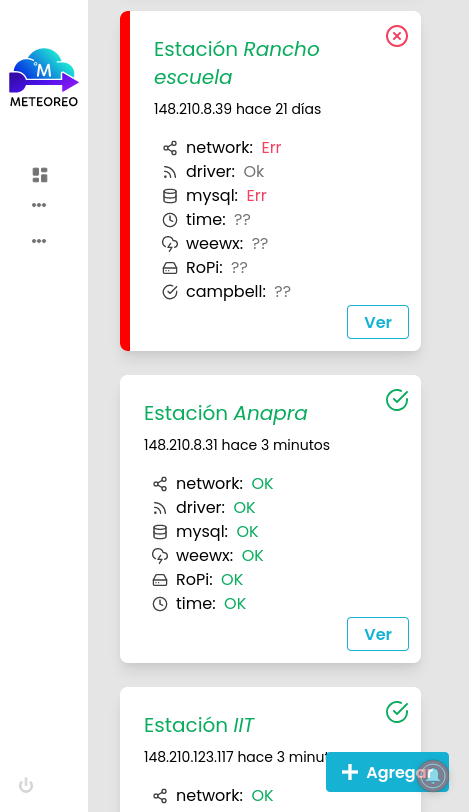
\includegraphics[width=0.37\linewidth]{images/screenshots/0.0.1-dashboard-responsive.png}
	\caption{Vista general en un celular.}
	\label{fig:dashboard-responsive}
\end{figure}

Posteriormente se desarrolló la vista de creado de una nueva estación, la cual se comunica con el API para tomar la información de la interfaz gráfica y enviarla, dicha interfaz se ve como puede ser observada en la Figura \ref{fig:reigster-station}. Al ser enviada, el API se conecta con el resto del sistema para dar de alta la estación, y de ser necesario el utilizar la información proveída para registrar la llave SSH en el sistema destino. Si este proceso es exitoso, se obtiene una respuesta satisfactoria y la interfaz es redirigida a la vista general de las estaciones, donde se puede observar la estación que se estaba registrando ya en el sistema.

\begin{figure}[!ht]
   \centering
   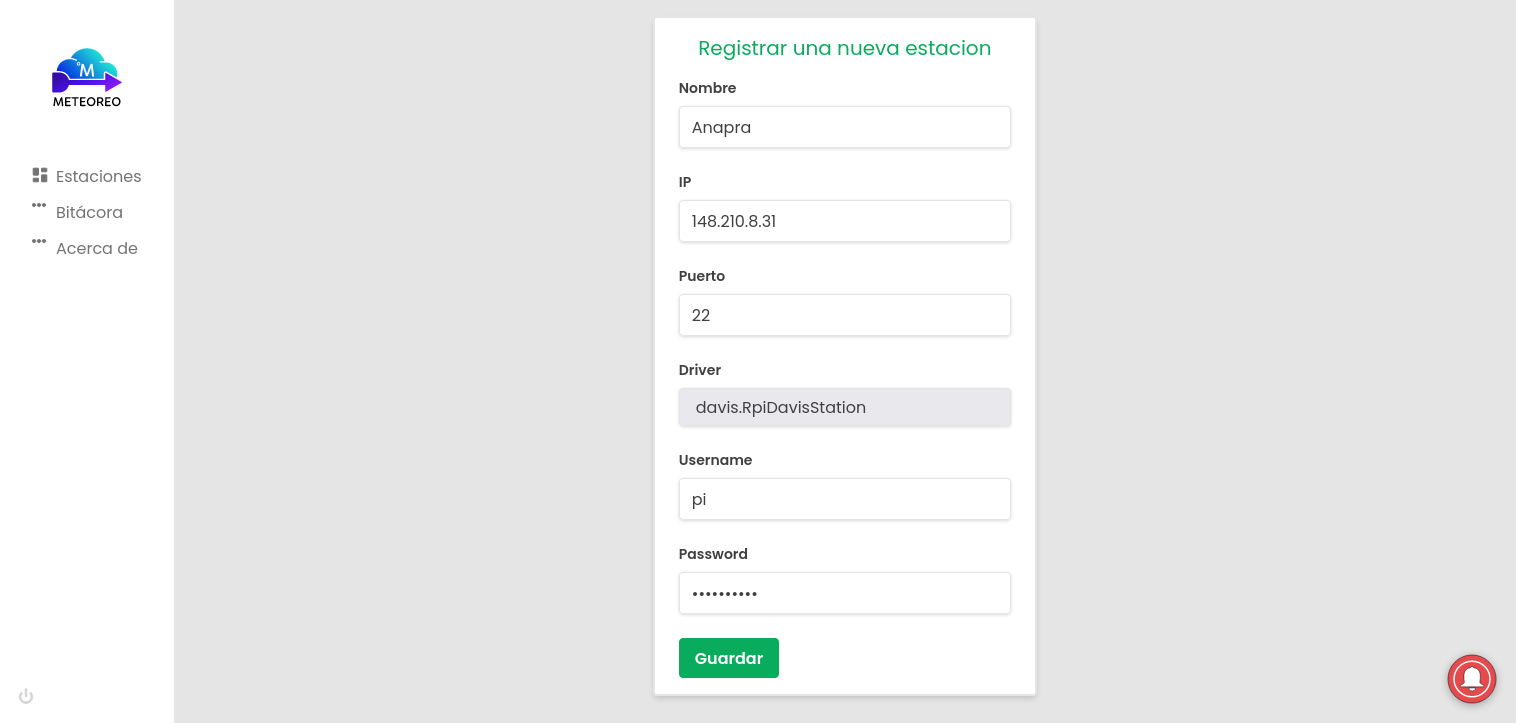
\includegraphics[width=1\linewidth]{images/screenshots/1.0.0-register_station.png}
   \caption{Vista de registro de una estación.}
   \label{fig:reigster-station}
\end{figure}

Una funcionalidad que no se encontraba contemplada al realizar el diseño inicial del sistema es la de tener una vista comprensiva de todos los eventos registrados en las estaciones que permitiera ver el historial de eventos completo, por lo tanto, se diseñó y se implementó una vista de bitácora. En esta vista, se agregó la funcionalidad de poder filtrar la información por diversos parámetros para poder realizar una evaluación rápida y precisa del sistema, así como eventualmente utilizar la información para generar reportes de calidad de los datos de los sistemas monitoreados, la pantalla resultante es la que se puede observar en la Figura \ref{fig:bitacora-filters}.

\begin{figure}[!ht]
   \centering
   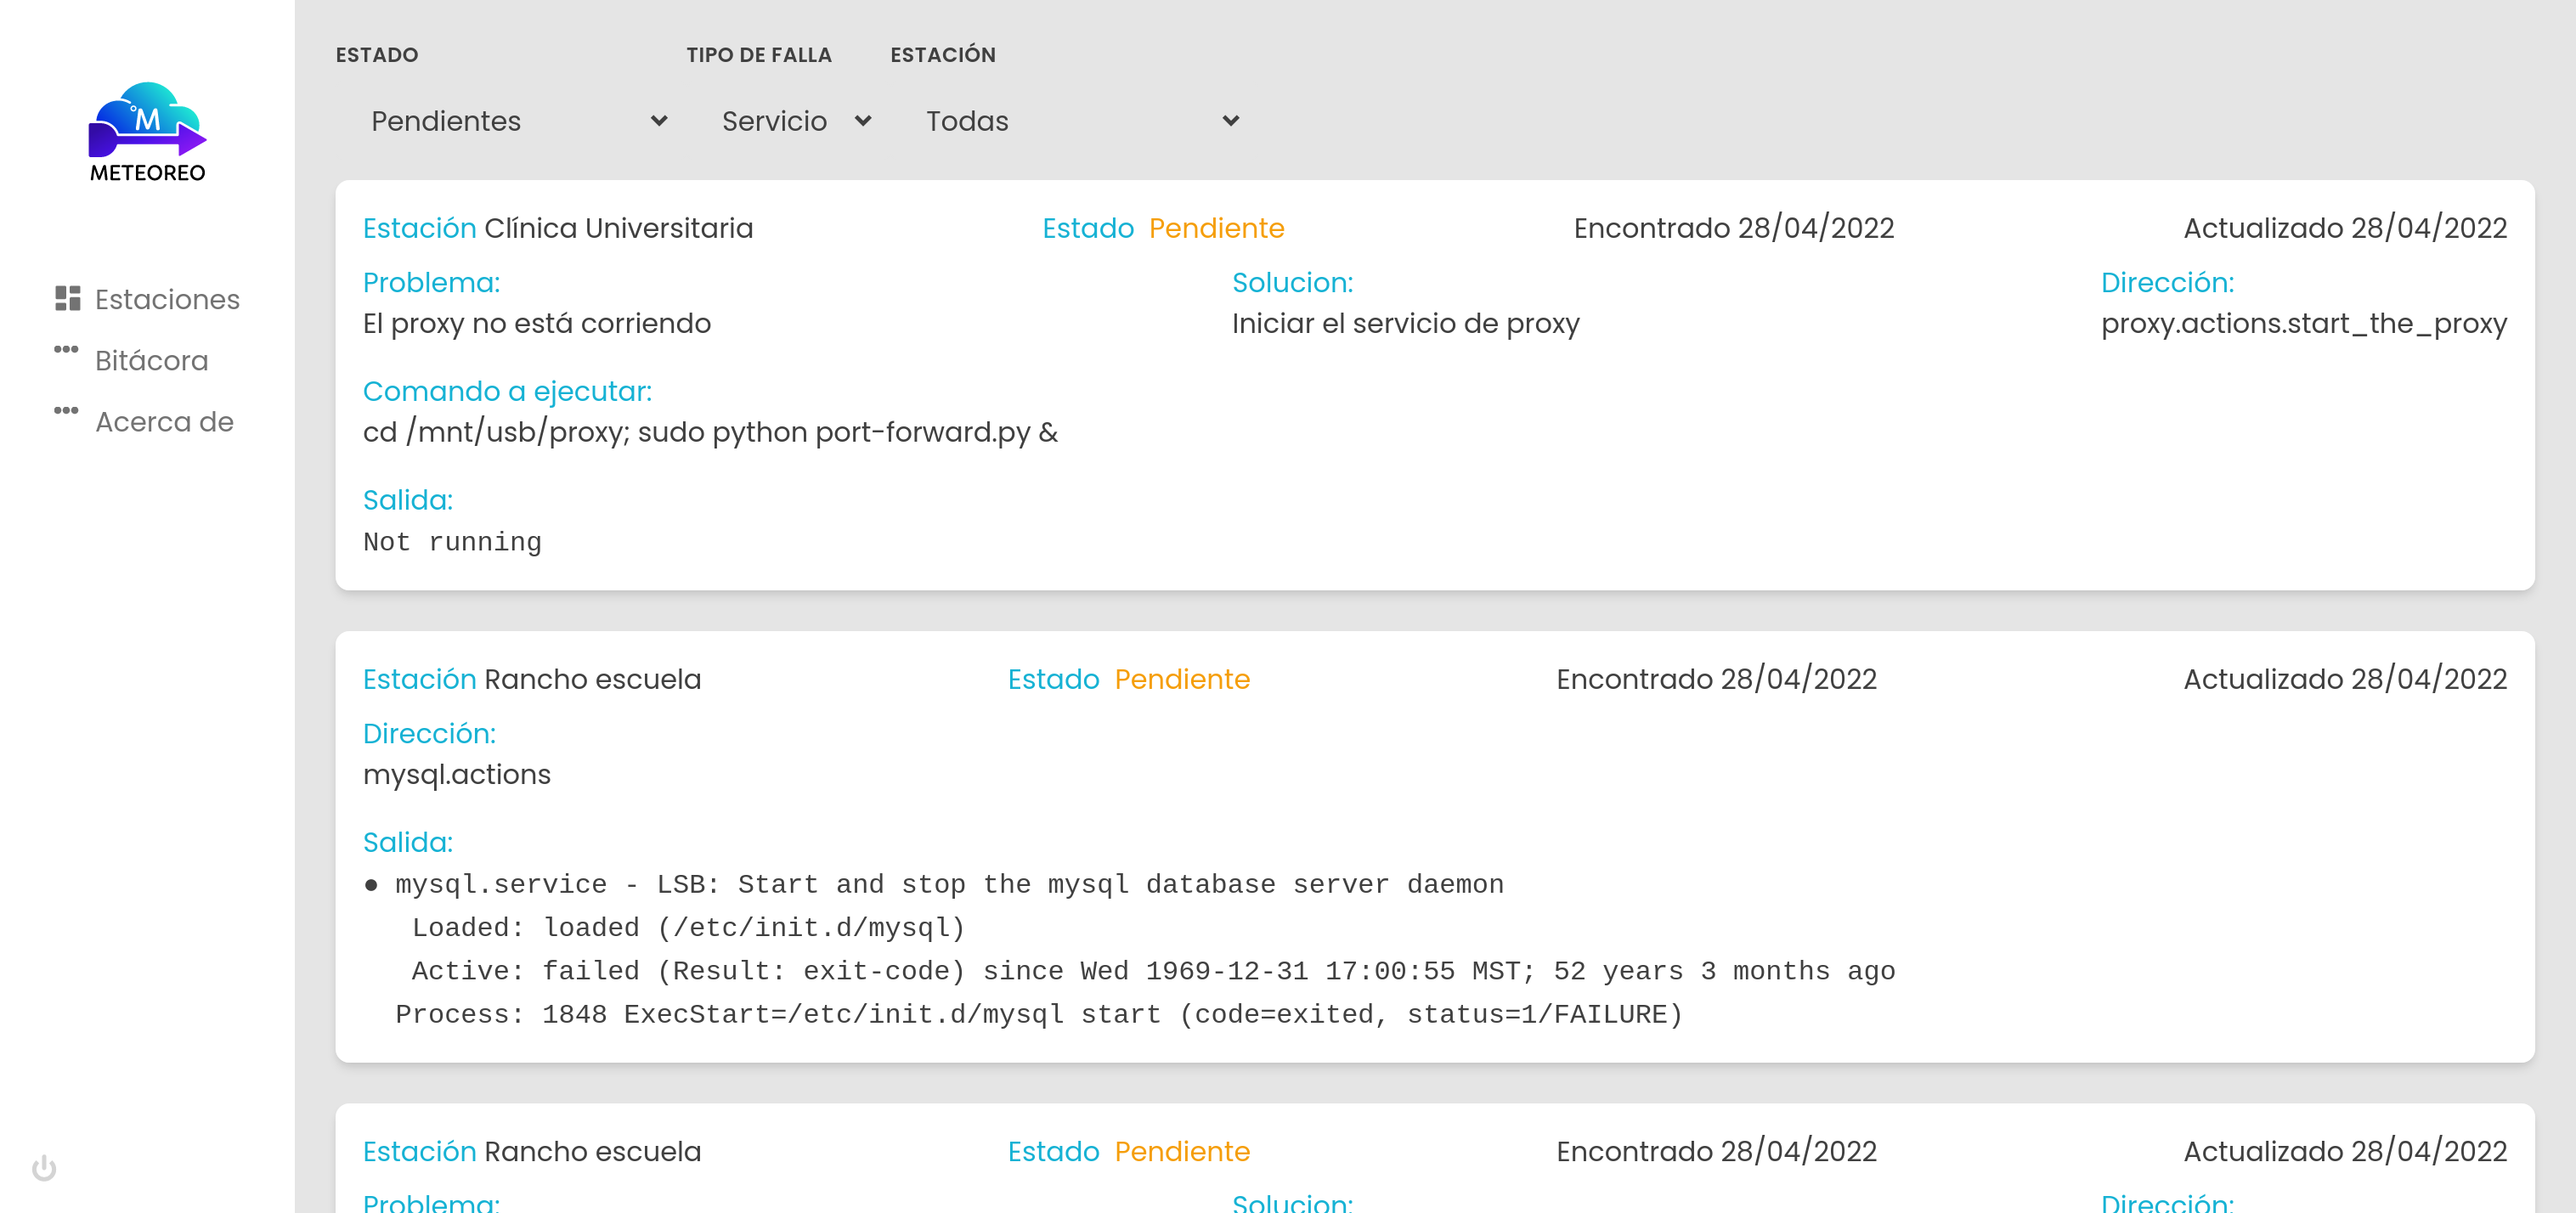
\includegraphics[width=1\linewidth]{images/screenshots/2.0.0-bitacora-filters.png}
   \caption{Vista de bitácora con filtros aplicados.}
   \label{fig:bitacora-filters}
\end{figure}

El sistema de autenticación que utiliza el proyecto está basado en el estándar \textit{HTTPBasic}, que sólo requiere de un usuario y contraseña para realizar operaciones en el sistema, el manejo de las operaciones de autenticación y de cerrado de sesión fueron posibles con un middleware creado gracias a la librería \textit{Axios}, la cual permite definir un preproceso a la información para tomar acciones correspondientes en el ambiente, como puede ser renovar un token de seguridad cuando se detecte que está próximo a expirar, o como lo es en este caso para agregar las cabeceras adecuadas para realizar la autenticación.

Por último, se integró el SDK de OneSignal, para ser integrado, sólo se requirió agregar las dependencias al sistema por medio de el gestor de paquetes npm, y seguir las instrucciones que aparecen al momento del registro. Debido a que el sistema se configuró para utilizar variables de entorno que fueran accesibles mientras se utiliza el sistema, fué posible especificar el \texttt{AppID} sin dejarlo escrito directamente en el código. Además de esto, se utilizaron opciones especiales para que el diálogo de notificaciones que aparece fuera diferente al original. El diálogo resultante es el que se puede observar en la Figura \ref{fig:onesignal-notifications-dialog} y el código relevante en el Listado \ref{lst:onesignal-configuration}.

\begin{listing}
\begin{minted}[%
   breaklines
]{js}
[...]
new Vue({
  router,
  render: h => h(App),
  beforeMount() {
    this.$OneSignal.init({
      appId: process.env.VUE_APP_ONESIGNAL_APP_ID,
      allowLocalhostAsSecureOrigin: true,
      autoRegister: false,
      notifyButton: {
        enable: true,
        size: 'medium',
        theme: 'default',
        position: 'bottom-right',
      }
    });
  },
}).$mount('#app')
\end{minted}
\caption{Serialización de datos con FastAPI y MasoniteORM.}
\label{lst:onesignal-configuration}
\end{listing}

\begin{figure}[!ht]
	\centering
	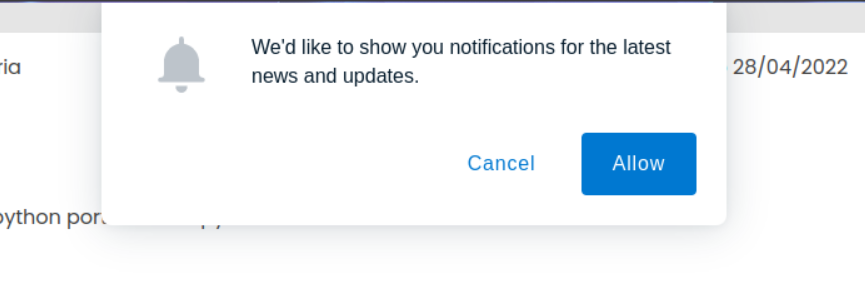
\includegraphics[width=0.7\linewidth]{images/screenshots/2.0.1-onesignal-notifications.png}
	\caption{Diálogo de notificaciones para OneSignal.}
	\label{fig:onesignal-notifications-dialog}
\end{figure}
